\part{kai}
\input{./preambel/table-of-content}
%hier gehts los

\section{TikZ}
\begin{frame}
\frametitle{Umgebung}
\begin{itemize}
  \item Zum Zeichnen unter \LaTeX wird nachfolgend TikZ verwendet
  \item die Zeichenumgebung wird mit $\backslash$ begin\{tikzpicture\} begonnen
\end{itemize}
\end{frame}

\begin{frame}
\frametitle{Kreise}
\begin{table}[!h]
\begin{tabular}{ccccc}
$\backslash$ path[draw] & & $\backslash$ path[fill] & & $\backslash$ path[fill=yellow, draw=red] \\
\\

\begin{tikzpicture}
  \path[draw] (0,0) circle (2ex);
\end{tikzpicture} 
& &

\begin{tikzpicture}
  \path[fill] (0,0) circle (2ex);
\end{tikzpicture}
& &

\begin{tikzpicture}
  \path[fill=yellow,draw=red] (0,0) circle (2ex);
\end{tikzpicture}
\\
\end{tabular}
\end{table}
\end{frame}

\begin{frame}
\frametitle{Diagramme}
\begin{figure}[!h]
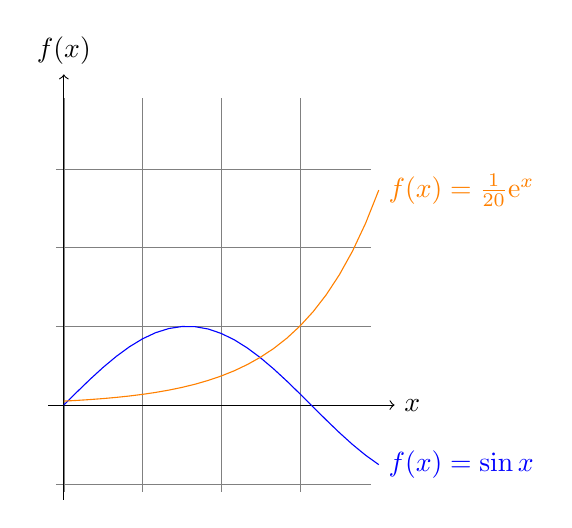
\begin{tikzpicture}[domain=0:4]
\draw[very thin,color=gray] (-0.1,-1.1) grid (3.9,3.9);
\draw[->] (-0.2,0) -- (4.2,0) node[right] {$x$};
\draw[->] (0,-1.2) -- (0,4.2) node[above] {$f(x)$};
\draw[color=blue] plot (\x,{sin(\x r)}) node[right] {$f(x) = \sin x$};
\draw[color=orange] plot (\x,{0.05*exp(\x)}) node[right] {$f(x) = \frac{1}{20} \mathrm e^x$};
\end{tikzpicture}
\end{figure}

\end{frame}
